%!TEX root = ../Thesis.tex
\section{Einleitung}

\subsection{Aufbau und Vorgehen}
Die Ausarbeitung gliedert sich in sieben Kapitel. Das erste Kapitel \textit{Vorwort und Motivation} dient der Hinführung in das Thema und der Motivation. Im \textit{Abstract} wird eine kurze Zusammenfassung über das Ziel, verwendete Methoden und Ergebnisse der Bachelorarbeit gegeben.

Das Kapitel \textit{Einleitung} führt grundsätzlich in das Thema ein. Dafür wird im ersten Teil das Partnerunternehmen Bertelsmann SE \& Co. KGaA und die Tochtergesellschaft \gls{AFS} mit ihrem Inkassounternehmen \gls{IFM} vorgestellt. Im zweiten Teil der Einleitung wird die Ist-Situation und das bestehende Problem beschrieben. Darauf folgen die \textit{Zielsetzung, Forschungsfrage und Hypothesen}, die es am Ende der Arbeit zu beantworten und zu überprüfen gilt. 

Im darauf folgenden Kapitel geht es darum, die benötigten theoretischen \textit{Grundlagen} zu erklären. Dafür wird auf die \textit{eingesetzten Technologien} und Werkzeuge, die im Projektgeschehen benutzt werden, eingegangen. Im Anschluss folgt der thematische Einstieg in die \textit{Software-Ergonomie} zu der einige Begriffe definiert und \textit{Gestaltgesetze, Normen, Richtlinien, Verordnungen} sowie \textit{Heuristiken} zum Designen von Benutzeroberflächen vorgestellt werden. 

Im Kapitel \textit{Evaluation von Software-Ergonomie} werden zuerst verschiedene Zieldefinitionen und die zwei \textit{Arten der Evaluation} vorgestellt. Im Anschluss werden dann, die für das Projekt relevanten, \textit{Erhebungsmethoden} erläutert. Zu diesen werden einzelne Vor- und Nachteile sowie \textit{Gütekriterien}, anhand derer die Qualität der Erhebung gemessen wird, genauer beleuchtet. Zuletzt wird auf \textit{Grundbegriffe}, die im Kontext der \textit{Statistik} eine Rolle spielen, eingegangen.

Im anschließenden Kapitel wird der Ansatz des \textit{Usability-Engineerings} erläutert. In dem Zusammenhang wird ein \textit{Vorgehensmodell} sowie \textit{Analysemethoden} vorgestellt und der Begriff \textit{Nutzungskontext} genauer betrachtet. 

In Kapitel fünf \textit{Entwicklung der neuen Benutzeroberfläche für Vermögensauskünfte} geht es darum die neue Benutzerschnittstelle für Vermögensauskünfte, mit Hilfe der Empfehlungen und Vorgaben aus Kapitel 4.2, zu konzipieren und für einen produktiven Test zu implementieren. Dabei wird das \textit{Vorgehensmodell für den Entwicklungsprozess}, das in Kapitel \ref{sec:vorgehensmodellUsabilityEngineering} vorgestellt wird, auf den Projektkontext angewandt.

In dem Kapitel \textit{Evaluation} wird das Ziel und der Aufbau der Evaluation festgelegt. Für die anschließende Durchführung der \textit{empirische Datenerhebung} werden zunächst die eingesetzten \textit{Erhebungsmethoden} und \textit{Messinstrumente} bestimmt.

Im Anschluss an die empirische Erhebung werden Ergebnisse präsentiert, interpretiert und diskutiert. Dazu werden zunächst die erhobenen Daten, bezogen auf ihre Erhebungsmethode bzw. Analysemethode, ausgewertet und anschließend in einer Zusammenfassung auf gegenseitige Einflüsse und Wirkungen untersucht. Schlussendlich werden in der Zusammenfassung die Ziele, Hypothesen und die Forschungsfrage erneut aufgegriffen und beantwortet bzw. überprüft.

Im abschließenden Kapitel wird mit Hilfe der erzielten Ergebnisse ein \textit{Resümee und Ausblick} zur Ausarbeitung selbst und zu weiterfolgenden Projekten und Handlungsalternativen gegeben.


%%%%%%%%%%%%%%%%%%%%%%%%%%%%%%%%%%%%%%%%%%%%%%%%%%%%%%%%%%%%%%%%%%%%%%%%%%%%

\subsection{Unternehmensvorstellung}
\subsubsection{Bertelsmann SE \& Co. KGaA} Die Bertelsmann SE \& Co. KGaA (im folgenden nur noch als Bertelsmann bezeichnet) ist ein international branchenübergreifender Konzern. Der Hauptsitz liegt in Gütersloh und geht zurück auf den Drucker und Buchbinder Carl Bertelsmann, der 1835 den damaligen Buchverlag Bertelsmann gründete. Inzwischen hat sich der Verlag zu einem weltweit tätigen Medien-, Dienstleistungs- und Bildungsunternehmen, unter der Führung des Vorstandsvorsitzenden Thomas Rabe und dem Aufsichtsratvorsitzenden Christoph Mohn, weiterentwickelt\footnote{\cite{BertelsmannGeschaeftsbericht2016}}. Bertelsmann beschäftigt rund 119.000 Mitarbeiter (Stand: Juni 2018) und erwirtschaftete im Jahr 2017 einen Konzernumsatz von 17,2 Milliarden Euro\footnote{\cite{BertelsmannAufEinenBlick2018}}. Zu den wichtigsten Geschäftsbereichen und Tochtergesellschaften zählen die RTL Group, Penguin Random House, Gruner + Jahr, BMG, Arvato, die Bertelsmann Printing Group, die Bertelsmann Education Group und Bertelsmann Investments. Die Tochtergesellschaft Arvato, die zu 100\% zu Bertelsmann gehört, bietet beispielsweise Services und Lösungen im Bereich Finanzen, \gls{CRM}, \gls{SCM} und IT für Unternehmen rund um den Globus an\footnote{\cite{BertelsmannGeschaeftsbericht2016}}.

%%%%%%%%%%%%%%%%%%%%%%%%%%%%%%%%%%%%%%%%%%%%%%%%%%%%%%%%%%%%%%%%%%%%%%%%%%%%

\subsubsection{Forderungsmanagement der Arvato Financial Solutions}
Eine der Tochtergesellschaften im Bereich der Finanzdienstleistungen ist die \gls{AFS}. Die \gls{AFS} hat mit der \gls{IFM} ein Unternehmen, das im Bereich des Forderungsmanagements tätig ist. Dazu gehört, dass die \gls{IFM} für externe Unternehmen (Mandanten) Mahnprozesse im Inkassoverfahren übernimmt. Ein weiteres Produkt der \gls{AFS} ist der Ankauf von fremden Forderungen, dessen anfallende Eintreibungsprozesse und das damit verbundene finanzielle Risiko übernommen werden. 

\textbf{Infoscore Forderungsmanagement GmbH}

Die \gls{IFM} selber unterteilt sich in weitere Bereiche von denen die IT Collection Germany einer ist. Die Aufgabengebiete werden innerhalb des Bereichs auf die Abteilungen Architekturmanagement, Softwareentwicklung, Qualitätsmanagement, Operations, Infrastruktur und Shared Services aufgeteilt (siehe Abb. \ref{fig:organisationsstruktur}). Innerhalb der Abteilungen IT Softwareentwicklung und IT Operations sind die Aufgaben auf mehrere Teams aufgeteilt von denen jedes Team einen Zuständigkeitsbereich verantwortet. 
\begin{figure}[H]
  \centering
  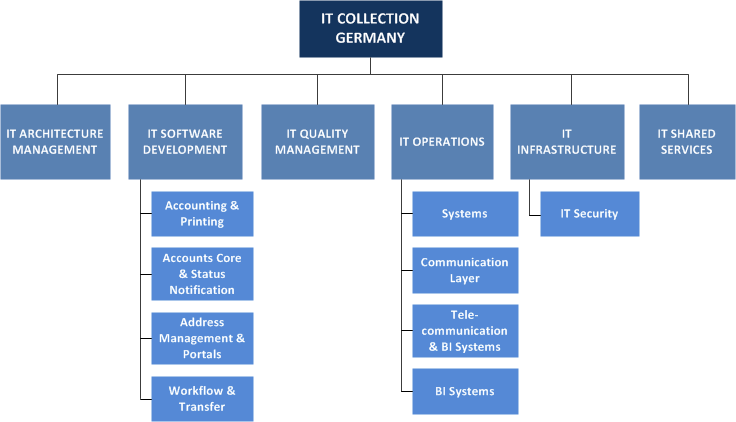
\includegraphics[scale=0.8]{img/IT_Collection_Germany_Organisation.png}
  \caption{Organisationsstruktur IT Collection Germany}
  \caption*{\textbf{Quelle:} Eigene Darstellung}
  \label{fig:organisationsstruktur}
\end{figure}

Weitere Bereiche sind die fachspezifischen Bereiche. Dort wird ebenfalls zwischen Abteilungen und zugehörigen Teams unterschieden. Es gibt Teams, die nur Forderungen eines gewissen Mandanten bearbeiten oder Teams wie das Special Research Team (SRT), das sich um die Ermittlung wichtiger Informationen zum Schuldner kümmert. Jeder Fachbereich hat abhängig von seinem Zuständigkeitsbereich nur auf gewisse Forderungen und Oberflächen im System Zugriff.

\textbf{Inkassosoftware Cosima}

Die digitale Prozessunterstützung wird von der eigens entwickelten Client-Server-Anwen-dung Cosima übernommen. Die Anwendung basiert auf der Programmiersprache Java, daher wurde die grafische Oberfläche komplett mit Java-Swing\footnote{Eine Standardbibliothek der Java-Laufzeitumgebung zur Entwicklung von grafischen Oberflächen} entworfen. Mittlerweile besteht Cosima aus mehreren einzelnen Services und einer Client-Anwendung, die jedem Sachbearbeiter zur Verfügung steht. Cosima wurde ursprünglich am Entwicklerstandort Baden-Baden konzipiert und entwickelt.

Die Inkassosoftware findet in den verschiedensten Fachbereichen und Prozessabläufen anwendung. Cosima wird zum einen als Speichermedium für benötigte Mandanteninformationen, sowie jeglich rechtlich erlaubte und für den Inkassoprozess benötigte Informationen zu Forderungen und Schuldnern verwendet. Zum anderen unterstützt die Software die Sachbearbeiter bei ihrer täglichen Arbeit. 

Durch den ständigen Wandel von Gesetzen, Richtlinien und Anforderungen, muss Cosima durchgehend angepasst und erweitert werden. Darunter leidet auch die Qualität. Mit Blick auf die Performance und die damit verbundene Software-Ergonomie werden daher immer wieder IT getriebene Softwareprojekte ins Leben gerufen, bei denen es darum geht die Softwarequalität zu steigern. So kümmert sich besonders das Qualitätsmanagement darum, dass während des Entwicklungsprozesses gewisse Richtlinien und Normen eingehalten werden. Außerdem werden bestehende Benutzeroberflächen, die den Anforderungen nicht mehr gerecht werden, weil sie unübersichtlich oder ineffizient sind, nach und nach renoviert.

%%%%%%%%%%%%%%%%%%%%%%%%%%%%%%%%%%%%%%%%%%%%%%%%%%%%%%%%%%%%%%%%%%%%%%%%%%%%

\subsection{Ist-Situation und Problemstellung}
Durch zusätzliche Features und Anforderungen ist Cosima mit der Zeit immer weiter gewachsen. Meist bestehen solche Features aus einer erweiterten Datenstruktur und letztendlich einer Veränderung, Anpassung beziehungsweise Erweiterung von Benutzerschnittstellen. Cosima besitzt über achthundert verschiedene Dialoge zur Anzeige und Bearbeitung von Daten. Einer dieser Dialoge ist für die Verwaltung von Schuldnerinformationen zuständig. Genauer gesagt werden dort Informationen zur Lebenssituation, Finanzsituation und dem Vermögen eines Schuldners gespeichert. Die Oberfläche wird mittlerweile für mehr als nur einen Anwendungsfall eingesetzt und besitzt daher einige Bedien- und Eingabeelemente, die für den ursprünglichen Use-Case unrelevant sind. Dadurch, dass der Dialog für mehrere Anwendungsfälle verwendet wird aber nicht jeder Anwendungsfall die kompletten Daten aus dem Dialog benötigt, entsteht ein Overhead\footnote{Daten, die nicht zu den primären Nutzdaten zählen}, der das Arbeiten mit dem Dialog unnötig verkompliziert. Sachbearbeiter finden den Dialog inzwischen sehr unübersichtlich und die Benutzung eher schwerfällig und ineffizient.

Einer dieser Anwendungsfälle (siehe Anhang \ref{sec:ablaufZwangsvollstreckung}) tritt immer dann auf, wenn Schuldner ihre ausstehenden Forderungen nicht begleichen möchten oder nach eigenen Angaben nicht können. In diesen Fällen wird dann eine Zwangsvollstreckung eingeleitet. Dazu wird der Schuldner von einem, durch die \gls{AFS} beauftragten Gerichtsvollzieher, aufgesucht, um einen Vermögensantrag bzw. Vermögensverzeichnis (siehe Beispielformular im Anhang \ref{sec:beispielVermoegensverzeichnisFormular}) zu seiner aktuellen Lebens- und Finanzsituation auszufüllen. Dieser Antrag besitzt einen standardisierten Aufbau und wird, nachdem er vom Schuldner ausgefüllt wurde, an die \gls{AFS} geschickt. Als nächstes wird durch das System automatisch ein Listeneintrag\footnote{Ein Arbeitsauftrag, der für Sachbearbeiter im System erscheint} erstellt, der einem zuständigen Sachbearbeiter zugeteilt wird. Im ersten Arbeitsschritt öffnet der Mitarbeiter das, als PDF vorliegende, Dokument auf einem seiner Monitore. Gleichzeitig öffnet er den Dialog für Schuldnerinformationen auf einem weiteren Monitor. Nach und Nach werden dann die vorliegenden Angaben aus dem Vermögensantrag in den Dialog übernommen und am Ende abgespeichert.

Das Problem speziell in diesem Fall liegt darin, dass der Sachbearbeiter für zwei untereinander folgenden Informationen aus dem Antrag teilweise an mehrere verschiedenen Stellen in dem Dialog springen muss, um diese zu übernehmen. Der Arbeitsablauf wird durch solche Sprünge unterbrochen und der Bearbeiter muss sich häufig neu orientieren. Zudem ist der Dialog mit zunehmender Anzahl an Bedienelementen, auch immer unübersichtlicher geworden. Sachbearbeiter berichten immer wieder von einer zu komplexen und ineffizienten Benutzeroberfläche. Grundsätzlich brauchen auch neue Arbeitskräfte bei der Einarbeitung mit diesem Dialog länger als gewünscht. Der aktuelle Dialog ist in die Jahre gekommen und entspricht nicht mehr den Anforderungen der Verantwortlichen. Aus diesen Gründen sind sich die Beteiligten einig, dass eine Veränderung durchgeführt werden muss.

%%%%%%%%%%%%%%%%%%%%%%%%%%%%%%%%%%%%%%%%%%%%%%%%%%%%%%%%%%%%%%%%%%%%%%%%%%%%

\subsection{Zielsetzung, Forschungsfrage und Hypothesen}
Die Ist-Situation inklusive ihrer Problemstellung, dient als Ansatzpunkt für mein Projektziel, das sich in zwei Unterziele aufteilt. Der erste Teil des Ziels besteht aus der Konzeption und Implementierung eines neuen Dialogs für die Eingabe von Vermögensverzeichnissen bzw. -anträgen. Im zweiten Schritt soll dieser Dialog mit dem bestehenden Dialog für Vermögensverzeichnisse auf Basis einer empirischen Evaluation in den Disziplinen Ergonomie bzw. Effektivität, Effizienz und Benutzerzufriedenheit verglichen werden. Am Ende soll ein neuer Dialog zur Verfügung stehen, der dem Sachbearbeiter eine ergonomische, anwendungsfallorientierte und performante Eingabe von Vermögensverzeichnissen ermöglicht. Dabei soll dieses Projekt als erster Schritt für die Ablösung des alten Dialoges dienen. 

Im Verlauf der Abschlussarbeit gilt es, das zu erreichende Ziel, auch hinsichtlich aufgestellter Hypothesen und Antithesen zu überprüfen. Neben den Thesen gibt es eine zentrale Forschungsfrage, die mit den gewonnen Erkenntnissen und Ergebnissen am Ende der Thesis beantwortet werden soll. Die Hauptfrage mit der sich beschäftigt werden soll lautet: \enquote{Weist der neue Eingabedialog für Vermögensverzeichnisse eine höhere Gebrauchstauglichkeit auf als der alte Dialog?}.

Zusätzlich zu der Forschungsfrage werden drei Hypothesen aufgestellt, die im Ergebnisteil überprüft werden sollen. Die Hypothesen bzw. deren Antithesen dienen später als Hilfe bei der Beantwortung der Forschungsfrage. Die Nullhypothesen werden mit H1\textsubscript{0}, H2\textsubscript{0} und H3\textsubscript{0} deklariert und die entsprechenden Antithesen mit H1\textsubscript{A}, H2\textsubscript{A} und H3\textsubscript{A}. Eine der zu verifizierenden Hypothesen in diesem Kontext heißt H1\textsubscript{0}: \enquote{Wenn der neue Dialog verwendet wird, dann sinkt die durchschnittliche Bearbeitungszeit pro Bearbeitungsvorgang}. Dabei definiert sich ein Bearbeitungsvorgang als Eingabe der Daten eines Vermögensverzeichnisses in die Oberfläche. Eine weitere damit verbundene Hypothese lautet H2\textsubscript{0}: \enquote{Mit dem neuen Dialog sinkt die durchschnittliche Anzahl von Interaktionen pro Bearbeitungsvorgang auf der Oberfläche}. Im Bereich der Ergonomie wird die Hypothese H3\textsubscript{0}: \enquote{Der neue Dialog wird im Gegensatz zum alten Dialog als ergonomischer empfunden} aufgestellt. Zudem werden diese Hypothesen ebenfalls als zu untersuchenden Antithesen umformuliert H1\textsubscript{A}: \enquote{Wenn der neue Dialog verwendet wird, dann stagniert oder steigt die durchschnittliche Bearbeitungszeit pro Bearbeitungsvorgang}, H2\textsubscript{A}: \enquote{Mit dem neuen Dialog steigt die durchschnittliche Anzahl von Interaktionen pro Bearbeitungsvorgang auf der Oberfläche} und H3\textsubscript{A}: \enquote{Der neue Dialog wird im Gegensatz zum alten Dialog als gleich bzw. weniger ergonomisch empfunden}.

%%%%%%%%%%%%%%%%%%%%%%%%%%%%%%%%%%%%%%%%%%%%%%%%%%%%%%%%%%%%%%%%%%%%%%%%%%%%




